\chapter{Application}
\label{chap:application}
%#############################################################################################

In this chapter, the implementations should be applied to three datasets: \textit{2gaussians} dataset, \textit{5gaussians} and \textit{USPS} dataset.

%#############################################################################################
\section{Assignment 6: \textit{5gaussians} Analysis}
\label{assignment6}

In this assignment, the \textit{5gaussians} data set is analyzed. The data set should be clustered using \textit{k-means} and \textit{GMM} for $k = 2, ..., 10$. Figure~\ref{fig:5gaussians} shows the original \textit{5gaussians} data set. Since the data set is constructed with five gaussians, $k=5$ is the best choice for the number of clusters.

\begin{figure}[h!]
	\centering
	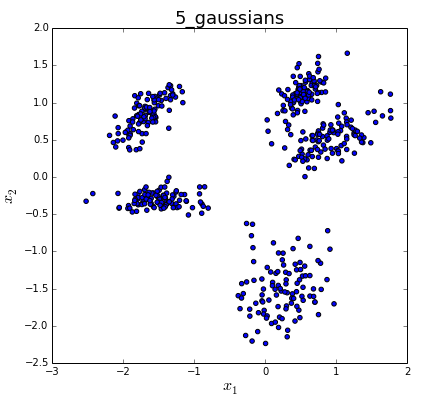
\includegraphics[scale=0.5983]{5gaussians}
	\caption{\textit{5gaussians} data set}
	\label{fig:5gaussians}
\end{figure}

{\raggedright \textbf{Question 6.1: Do both methods find the five clusters reliably?}} \\
\textit{K-means} finds the five clusters reliably. Since \textit{k-means} can have different result depending on the initialization, it was run 100 times. The loss value from each run was calculated, as depicted in Figure~\ref{fig:lossvalues_kmeans}. The clustering which gives the lowest loss value was then picked and visualized in Figure~\ref{fig:5gaussians_kmeans}.

\begin{figure}[h!]
	\centering
	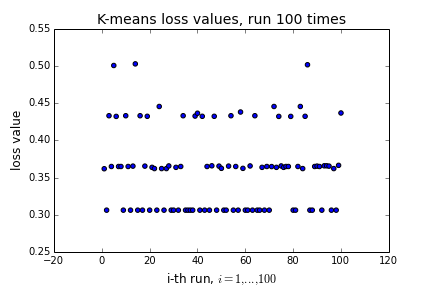
\includegraphics[scale=0.5983]{lossvalues_kmeans}
	\caption{Loss values of k-means, run 100 times}
	\label{fig:lossvalues_kmeans}
\end{figure}

\begin{figure}[h!]
	\centering
	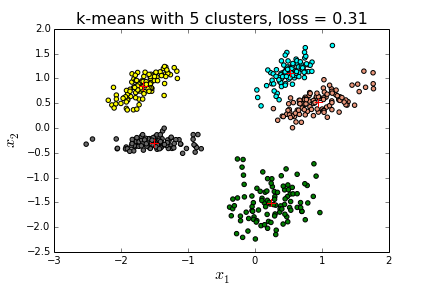
\includegraphics[scale=0.5983]{5gaussians_kmeans}
	\caption{k-means clustering with $k=5$, applied to \textit{5gaussians} data set}
	\label{fig:5gaussians_kmeans}
\end{figure}

\textit{GMM} with random initialization also finds the five clusters reliably. The same method as \textit{k-means} was applied to \textit{GMM}. It was also run 100 times, but instead of loss value, the log likelihood of each run was calculated, as shown in Figure~\ref{fig:likelihoods_gmm_random}. The clustering which gives the highest log likelihood was then picked and visualized in Figure~\ref{fig:5gaussians_gmm_random}.

\begin{figure}[h!]
	\centering
	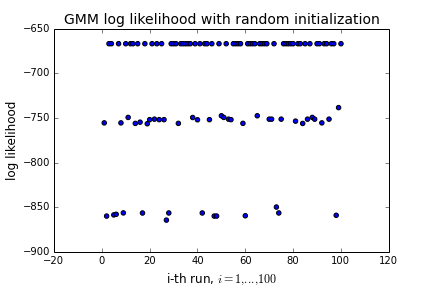
\includegraphics[scale=0.5983]{likelihoods_gmm_random}
	\caption{Log likelihood of GMM with random initialization, run 100 times}
	\label{fig:likelihoods_gmm_random}
\end{figure}

\begin{figure}[h!]
	\centering
	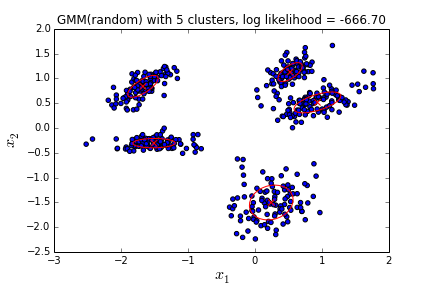
\includegraphics[scale=0.5983]{5gaussians_gmm_random}
	\caption{GMM clustering with random initialization, $k=5$, applied to \textit{5gaussians} data set}
	\label{fig:5gaussians_gmm_random}
\end{figure}

Finally, \textit{GMM} with \textit{k-means} initialization was utilized. It also finds the five clusters reliably. It was also run 100 times and the log likelihood of each run was calculated. Figure~\ref{fig:likelihoods_gmm_kmeans} and Figure~\ref{fig:5gaussians_gmm_kmeans} depict the log likelihood of each run and the clustering which gives the highest log likelihood, respectively.

\begin{figure}[h!]
	\centering
	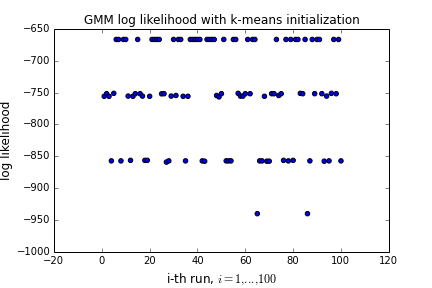
\includegraphics[scale=0.5983]{likelihoods_gmm_kmeans}
	\caption{Log likelihood of GMM with k-means initialization, run 100 times}
	\label{fig:likelihoods_gmm_kmeans}
\end{figure}

\begin{figure}[h!]
	\centering
	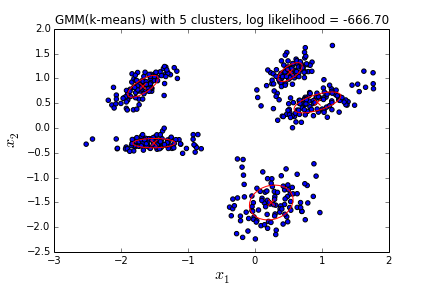
\includegraphics[scale=0.5983]{5gaussians_gmm_kmeans}
	\caption{GMM clustering with k-means initialization, $k=5$, applied to \textit{5gaussians} data set}
	\label{fig:5gaussians_gmm_kmeans}
\end{figure}

As we have seen above, the three methods can find the five clusters reliably, because the \textit{5gaussians} data set is a well-separated data set.

%\newpage
\pagebreak[4]
{\raggedright \textbf{Question 6.2: What role does the initialization of the GMM with a k-means solution play in the number of necessary iterations and the quality of the solution?}}\\

The initialization of the \textit{GMM} with a \textit{k-means} solution plays a significant role in the number of necessary iterations until the convergence is reached. \textit{GMM} depends strongly on the initialization. With \textit{k-means} initialization, the \textit{GMM} converged more quickly than random initialization.

\textit{GMM} was run 100 times with random and k-means initialization to avoid some bad local optima. As we can see from Figure~\ref{fig:number_iterations}, \textit{GMM} with random initialization never converged with the number of iterations below 20, whereas \textit{GMM} with k-means initialization converged mostly only with about eight iterations.

On the other hand, the initialization does not play a significant role in the quality of the solution. Both the random and k-means initialization produce almost the same log likelihoods. Figure~ shows the maximum log likelihoods of both initialization which were run 100 times. Both methods produce almost the same maximum log likelihood, about -666.7011.

\begin{figure}[h!]
	\centering
	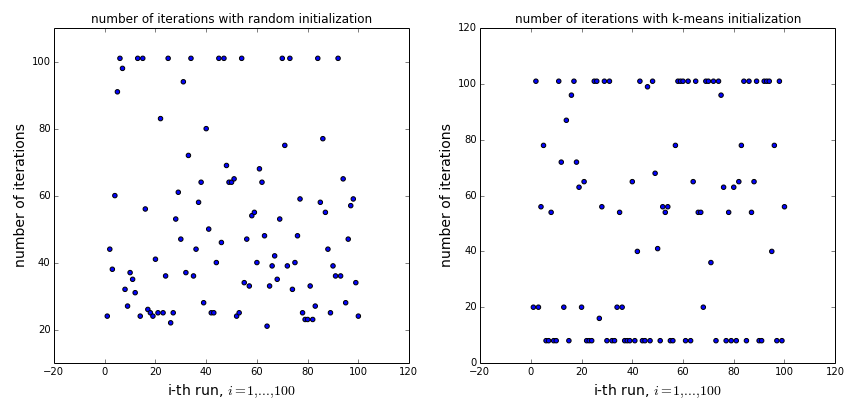
\includegraphics[scale=0.4783]{number_iterations}
	\caption{Number of iterations of \textit{GMM} ($k=5$) with random and k-means initialization, run 100 times}
	\label{fig:number_iterations}
\end{figure}

\begin{figure}[h!]
	\centering
	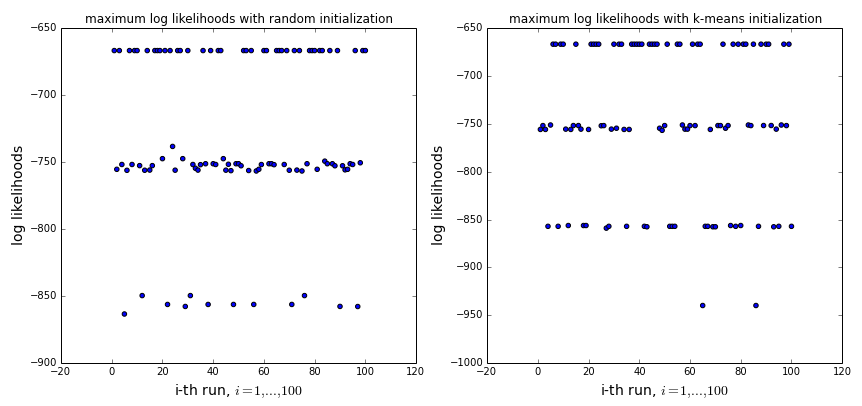
\includegraphics[scale=0.4783]{likelihoods_comparison}
	\caption{Maximum log likelihoods of \textit{GMM} ($k=5$) with random and k-means initialization, run 100 times}
	\label{fig:likelihoods_comparison}
\end{figure}


{\raggedright \textbf{Question 6.3: What does the dendogramm of the hierarchical clustering look like and is it possible to pick a suitable value of \textit{k} from the dendogramm?}}\\

It is possible to pick a suitable value of \textit{k} from the dendogramm plot. Figure~\ref{fig:5gaussians_dendogramm_50clusters} shows the dendogramm plot of \textit{kmeans\_agglo} with initial clustering $k=50$. From the plot, we can see that the clusters can actually be divided into five clusters (marked with yellow ellipses). Before the merge of those five clusters, there is no significant increase of the loss values. But after merging those five clusters, the loss values increase significantly.

\begin{figure}[h!]
	\centering
	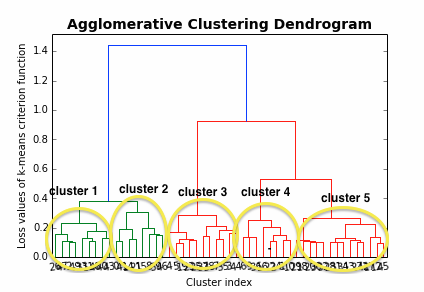
\includegraphics[scale=0.7583]{5gaussians_dendogramm_50clusters}
	\caption{Dendogramm plot of the hierarchical clustering with initial clustering $k=50$}
	\label{fig:5gaussians_dendogramm_50clusters}
\end{figure}

In this case the difference in iterations
seems insignificant. However, as will be seen in the presence of poorly separated data a good choice for our
initial guesses can drastically reduce the number of iterations required to obtain convergence


%#############################################################################################
\section{Assignment 7: \textit{2gaussian} Analysis}
\label{assignment7}

In this assignment the \textit{2gaussians} data set should be analyzed with \textit{k-means} and \textit{GMM}. Figure~\ref{fig:2gaussians} show the original \textit{2gaussians} data set. Since the data set is constructed by two gaussians, $k=2$ is the best choice for the number of clusters.

\begin{figure}[h!]
	\centering
	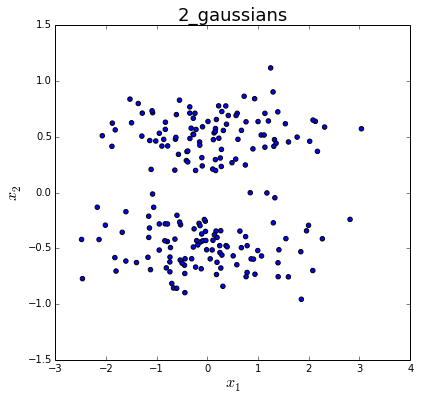
\includegraphics[scale=0.5983]{2gaussians}
	\caption{\textit{2gaussians} data set}
	\label{fig:2gaussians}
\end{figure}

{\raggedright \textbf{Question 7.1: Compare the cluster centers. Which algorithm works better and why?}}\\

\textit{K-means}, \textit{GMM} with random and k-means initialization were used to cluster the \textit{2gaussians} data set. Each method was run 100 times to avoid bad local optima. For \textit{k-means} method, the clustering which gives the lowest loss value was picked, whereas for \textit{GMM}, the clustering which gives the highest log likelihood was picked. Figure~\ref{fig:2gaussians_kmeans} shows the clustering using \textit{k-means}, whereas Figure~\ref{fig:2gaussians_gmm_random} and Figure~\ref{fig:2gaussians_gmm_kmeans} show the clustering using \textit{GMM} with random and k-means initialization.

\begin{figure}[h!]
	\centering
	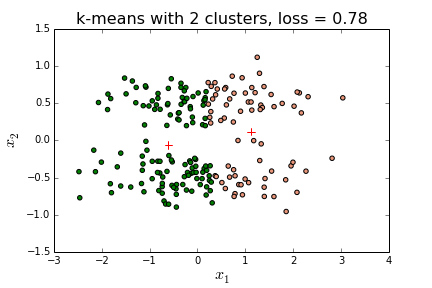
\includegraphics[scale=0.5983]{2gaussians_kmeans}
	\caption{k-means clustering with $k=2$, applied to \textit{2gaussians} data set}
	\label{fig:2gaussians_kmeans}
\end{figure}

\begin{figure}[h!]
	\centering
	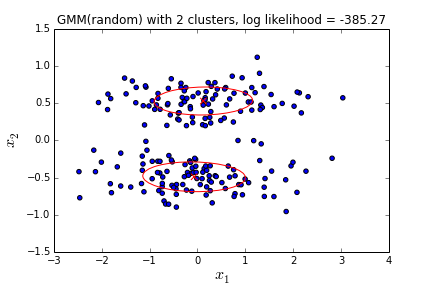
\includegraphics[scale=0.5983]{2gaussians_gmm_random}
	\caption{GMM clustering with random initialization, $k=2$, applied to \textit{2gaussians} data set}
	\label{fig:2gaussians_gmm_random}
\end{figure}

\begin{figure}[h!]
	\centering
	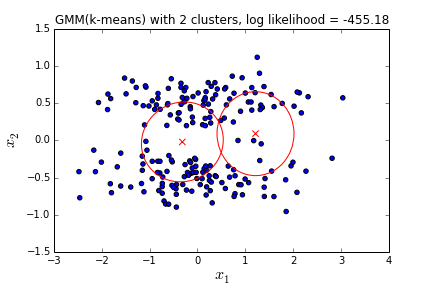
\includegraphics[scale=0.5983]{2gaussians_gmm_kmeans}
	\caption{GMM clustering with k-means initialization, $k=2$, applied to \textit{2gaussians} data set}
	\label{fig:2gaussians_gmm_kmeans}
\end{figure}

From the plots, it can be obtained that the \textit{GMM} with random initialization is the best method to cluster the \textit{2gaussians} data set. The \textit{k-means} method did not perform very well, because the objective of \textit{k-means} is to minimize the loss value, which basically depends strongly on the euclidean distances of each data point. But the data set was created using mixture of two gaussians which is separated as upper- and lower part. Therefore two data points can have a small euclidean distance although they are from two different gaussians. 

The \textit{GMM} with random initialization performed very well, because its objective is to maximize the log likelihood, which can be calculated using the gaussian function. Instead of depending on the mean of data points, it uses maximization to find the best clustering. On the other hand, the \textit{GMM} with k-means initialization did not perform very well, because \textit{GMM} depends strongly on the initialization. Since it used the result of k-means to do the initialization, it performed almost in the same way as k-means.

{\raggedright \textbf{Question 7.2: How does the GMM depends on the initialization}}\\

The \textit{GMM} depends strongly on the initialization, as we can see in the Figure~\ref{fig:2gaussians_gmm_random} and Figure~\ref{fig:2gaussians_gmm_kmeans}. Although the \textit{GMM} was applied to the same data set, but its performance was different, depending on the initialization.

%#############################################################################################

\section{Assignment 8: \textit{USPS} Analysis}
\label{assignment8}

In the last assignment of this problem set, the \textit{k-means} and \textit{GMM} algorithm should be applied to the \textit{USPS} data set with $k=10$.
